% 第2章第1节：线性映射与误差传递（定义域与有界性、算子空间、算子列的收敛）。

\section{线性映射与误差传递}
\label{sec:lfo-operators}

有限维中，矩阵$\bm A$作用于向量$\bm x$，输入的误差$\bm e$经过同一个矩阵变成输出误差$\bm A\bm e$。本节把这种作用推广到函数空间：先写清楚输入在哪个空间、输出在哪个空间、作用规则对哪些输入有意义，再用一个与输入无关的常数控制全部输入的误差。后面的泛函、伴随和逆算子都沿用这里的运算与连续性约定。

\subsection{线性算子的定义域与有界性}
\label{sec:lfo-boundedness}

\paragraph{三个作用规则}
先看三个熟悉的运算。第一个是加权积分：给定连续权重$w\geq0$，对$f\in C([0,1])$令$Wf=\int_0^1w(t)f(t)\,dt$，输入是连续函数，输出是一个实数。第二个是求导：对$u\in C^1([0,2\pi])$令$Du=u'$，输入必须可导，输出$u'$是连续函数。第三个是第~\ref{sec:fs-projection}节的正交投影：对Hilbert空间$H$的闭子空间$M$，令$P_M f$为$f$在$M$中的最近分量，输入和输出都在$H$中。

三个运算的输出形态各不相同，共同之处是它们都保持线性组合：两个输入先组合再作用，与先分别作用再组合，结果相同。差别还在于它们对输入的要求。积分和投影对空间中的每个元素都有意义，求导却只对可导函数有意义；若把求导看成从$C([0,2\pi])$出发的映射，就必须说明它只定义在一部分元素上。

\begin{definition}[线性算子与线性泛函]
\label{def:lfo-linear-operator}
设$X,Y$是同一标量域$\mathbb F$上的赋范空间，$D(A)\subset X$是线性子空间。映射$A:D(A)\to Y$若满足
\[
 A(\alpha x+\beta z)=\alpha Ax+\beta Az\qquad(x,z\in D(A),\ \alpha,\beta\in\mathbb F),
\]
则称$A$为从$X$到$Y$的\term{线性算子}（linear operator），$D(A)$称为它的\term{定义域}（domain）。$D(A)=X$时简记$A:X\to Y$。输出空间$Y=\mathbb F$时，称$A$为\term{线性泛函}（linear functional）。
\end{definition}

本章所说的算子，若不特别写出定义域，都定义在整个输入空间上。线性泛函是标量值的线性算子，因此下面关于算子的定义和结论都适用于泛函。

\paragraph{用一个常数控制全部输入}
线性使误差传递有一个简单形式：若输入$x$带有扰动$e$，则输出变为$A(x+e)=Ax+Ae$，输出误差只取决于扰动$e$本身，与$x$在哪里无关。于是问题化为：能否找到常数$C$，使任何扰动都满足$\|Ae\|\leq C\|e\|$？按线性把$e$缩放到单位长度，这等价于问单位球上的输出范数是否有统一上界。

\begin{definition}[有界线性算子与算子范数]
\label{def:lfo-operator-norm}
线性算子$A:X\to Y$若满足
\begin{equation}
 \|A\|=\sup_{\|x\|\leq1}\|Ax\|<\infty ,
 \label{eq:lfo-operator-norm}
\end{equation}
则称$A$为\term{有界线性算子}（bounded linear operator），$\|A\|$称为它的\term{算子范数}（operator norm）。
\end{definition}

由定义，对任意$x\neq0$有$\|A(x/\|x\|)\|\leq\|A\|$，乘回$\|x\|$得到
\begin{equation}
 \|Ax-Az\|=\|A(x-z)\|\leq\|A\|\,\|x-z\|\qquad(x,z\in X).
 \label{eq:lfo-lipschitz}
\end{equation}
$\|A\|$是使这一估计对一切输入成立的最小常数。“有界”说的是这个常数存在，不是说输出集合$\{Ax:x\in X\}$有界；非零线性算子的输出集合总是无界的。

\begin{theorem}[有界与连续等价]
\label{thm:lfo-bounded-continuous}
对线性算子$A:X\to Y$，下列三条等价：（i）$A$在$0$处连续；（ii）$A$在$X$上处处连续；（iii）$A$有界。
\end{theorem}

\begin{proof}
由式~\eqref{eq:lfo-lipschitz}，（iii）推出$A$是Lipschitz映射，因而（ii）成立；（ii）推出（i）是显然的。只需证明（i）推出（iii）。

取$\varepsilon=1$，由$A$在$0$处连续，存在$\delta>0$使$\|x\|\leq\delta$时$\|Ax\|\leq1$。对任意$\|x\|\leq1$，向量$\delta x$满足$\|\delta x\|\leq\delta$，于是$\|Ax\|=\delta^{-1}\|A(\delta x)\|\leq\delta^{-1}$。这说明$\|A\|\leq\delta^{-1}<\infty$。
\end{proof}

证明中关键的一步是缩放：线性算子在一个小球上的行为决定了它在所有尺度上的行为。因此对线性映射，“连续”和“有界”可以互换使用。

\paragraph{有限维中的最大伸长}
算子范数在平面上有直观的图像。取对称矩阵
\[
 \bm A=\begin{bmatrix}3/2&1/2\\1/2&3/2\end{bmatrix},
\]
它在方向$\bm v=(1,1)^{\top}/\sqrt2$上把长度放大为$2$倍，在正交方向$(1,-1)^{\top}/\sqrt2$上保持长度不变。单位圆在$\bm A$下的像是半轴为$2$和$1$的椭圆，如图~\ref{fig:lfo-operator-norm-stretch}所示。标准基向量$\bm e_1$被送到$(3/2,1/2)^{\top}$，长度只有$\sqrt{5/2}\approx1.58$；最大的伸长发生在$\bm v$方向，因此在欧氏范数下$\|\bm A\|=2$。有限维空间上任意两个范数等价，由此可知有限维空间上的线性映射总是有界的，可参考\BookChapterRef{chap:normed-inner-product-spaces}{卷一“赋范空间与内积空间”章}；无限维中这一点不再自动成立，下面的求导就是例子。

\begin{figure}[!htb]
  \centering
  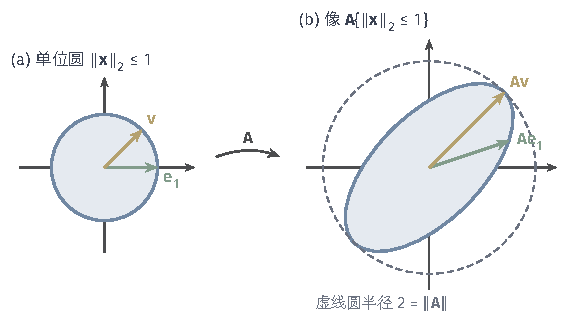
\includegraphics[width=95.1mm]{figures/02-abstract-mathematics/03-function-spaces/tikz/c2-operator-norm-stretch/figure.pdf}
  \caption{算子范数是单位球的像离原点最远的距离。(a)~平面单位圆及两个单位向量$\bm e_1$（绿）、$\bm v=(1,1)^{\top}/\sqrt2$（黄）；(b)~在$\bm A=\bigl[\begin{smallmatrix}3/2&1/2\\1/2&3/2\end{smallmatrix}\bigr]$作用下，单位圆变为旋转$45^\circ$、半轴为$2$与$1$的椭圆。$\bm A\bm e_1$的长度约为$1.58$，$\bm A\bm v$的长度为$2$，恰好触到半径为$\|\bm A\|=2$的虚线圆。}
  \label{fig:lfo-operator-norm-stretch}
\end{figure}

\paragraph{上确界未必取到}
在平面例子中，最大伸长由某个单位向量实际取到；无限维中，式~\eqref{eq:lfo-operator-norm}的上确界不一定是某个输入的输出。在$\ell^2$上令$A(x_1,x_2,x_3,\ldots)=\bigl(\tfrac12x_1,\tfrac23x_2,\tfrac34x_3,\ldots\bigr)$，即第$n$个坐标乘以$n/(n+1)$。每个坐标被乘以小于$1$的因子，故$\|Ax\|<\|x\|$对一切$x\neq0$成立；另一方面，标准单位向量满足$\|Ae_n\|=n/(n+1)\to1$，所以$\|A\|=1$，但没有任何单位向量使$\|Ax\|=1$。因此$\|A\|$应理解为“最小的统一上界”，不能无条件称为“最大输出”。

\paragraph{加权积分的范数}
回到加权积分$Wf=\int_0^1wf\,dt$，输入空间取$C([0,1])$配一致范数$\|f\|_\infty$。由$|Wf|\leq\int_0^1w|f|\,dt\leq\|f\|_\infty\int_0^1w\,dt$得$\|W\|\leq\int_0^1w\,dt$；取$f\equiv1$时等号成立，所以$\|W\|=\int_0^1w\,dt$。例如$w(t)=2t$时$\|W\|=1$。同一个读数规则若改用$L^2$范数衡量输入，算子范数会变成另一个数，第~\ref{sec:lfo-point-evaluation}节将用Hölder不等式计算。

\paragraph{求导：有界性取决于范数}
现在看求导$D$。若输入空间取$C^1([0,2\pi])$，并配上同时控制函数值与导数的范数
\[
 \|u\|_{C^1}=\|u\|_\infty+\|u'\|_\infty ,
\]
则$\|Du\|_\infty=\|u'\|_\infty\leq\|u\|_{C^1}$，$D:C^1([0,2\pi])\to C([0,2\pi])$是有界算子，$\|D\|\leq1$。取$u_n(x)=\sin(nx)/n$，有$\|Du_n\|_\infty=1$而$\|u_n\|_{C^1}=1+1/n$，比值趋于$1$，所以$\|D\|=1$；这个上确界同样不被取到，因为取到它需要$\|u\|_\infty=0$。

若在同一个函数集合$C^1([0,2\pi])$上只用一致范数$\|u\|_\infty$衡量输入，情况就完全不同。取$u_n(x)=\sin(nx)$，则
\[
 \|u_n\|_\infty=1,\qquad \|Du_n\|_\infty=\|n\cos(nx)\|_\infty=n .
\]
输出与输入的范数之比为$n$，可以任意大，所以不存在统一常数。图~\ref{fig:lfo-sine-derivative}显示了原因：振幅不变而频率升高时，函数值始终在$[-1,1]$中，斜率却按频率放大。输入上一个一致范数很小的高频扰动，可以使导数产生很大的误差。

\begin{figure}[!htb]
  \centering
  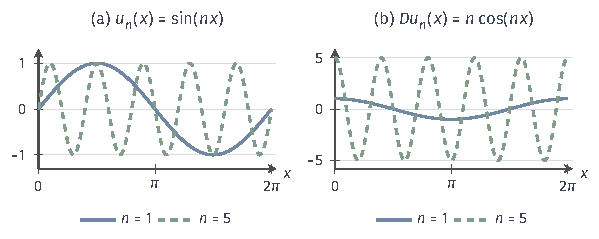
\includegraphics[width=101.5mm]{figures/02-abstract-mathematics/03-function-spaces/tikz/c2-sine-derivative/figure.pdf}
  \caption{求导对高频输入放大误差。(a)~$u_n(x)=\sin(nx)$在$n=1$（蓝实线）与$n=5$（绿虚线）时的一致范数都为$1$；(b)~导数$n\cos(nx)$的一致范数为$n$。若输入只用一致范数衡量，求导不存在统一的误差界；改用同时计入导数的$C^1$范数后，同一作用规则变为有界算子。}
  \label{fig:lfo-sine-derivative}
\end{figure}

这个例子说明，说一个算子是否有界时，必须同时交代三件事：作用规则、定义域以及定义域上的范数。把$D$看成从$C([0,2\pi])$到自身的算子时，它的定义域$D(D)=C^1([0,2\pi])$只是$C([0,2\pi])$的一个子空间，而且它在一致范数下无界，这类算子称为\term{无界算子}（unbounded operator）。对这类算子必须明确写出$D(A)$，不能把它当作已经定义在整个$X$上；第~\ref{sec:lfo-closed-graph}节还会回到求导，说明怎样选择定义域上的范数使它重新成为有界算子。

\subsection{算子的运算与算子空间}
\label{sec:lfo-operator-space}

\paragraph{加法、数乘与复合}
同一对空间之间的两个算子可以相加和数乘：对$A,B:X\to Y$及标量$\alpha$，令$(A+B)x=Ax+Bx$，$(\alpha A)x=\alpha Ax$。若$A:X\to Y$、$B:Y\to Z$，前者的输出空间正是后者的输入空间，就可以复合，$(BA)x=B(Ax)$，先作用$A$、再作用$B$，与矩阵乘积的顺序相同。这些运算都保持线性，问题是它们是否保持有界，以及范数怎样变化。

\begin{theorem}[算子运算的范数估计]
\label{thm:lfo-operator-algebra}
设$A,B:X\to Y$有界，$C:Y\to Z$有界，$\alpha\in\mathbb F$。则$A+B$、$\alpha A$与$CA$都有界，且
\[
 \|A+B\|\leq\|A\|+\|B\|,\qquad \|\alpha A\|=|\alpha|\,\|A\|,\qquad \|CA\|\leq\|C\|\,\|A\| .
\]
\end{theorem}

\begin{proof}
三个估计都先对单个输入成立，再对单位球取上确界。对$\|x\|\leq1$，由$Y$中的三角不等式，$\|(A+B)x\|\leq\|Ax\|+\|Bx\|\leq\|A\|+\|B\|$；数乘的等式直接来自范数的齐次性。复合时先用$C$的界，再用$A$的界：$\|C(Ax)\|\leq\|C\|\,\|Ax\|\leq\|C\|\,\|A\|$。
\end{proof}

复合的估计一般是严格不等式。在平面上取$\bm A=\operatorname{diag}(1,0)$、$\bm C=\operatorname{diag}(0,1)$，两者范数都是$1$，乘积却是零矩阵：$\bm A$保留的方向恰好被$\bm C$消去。每个空间都有自己的单位算子$I_X$和零算子，写复合时须分清它们属于哪个空间，例如$I_YA=A=AI_X$。

\paragraph{先投影再读数}
标量读数可以与一般变换使用同一套运算。在$H=L^2(0,1)$中，令$M$为常数函数组成的一维子空间。常数$1$是$M$中的单位向量，所以投影为$Pf=\langle1,f\rangle\cdot1=\bigl(\int_0^1f\,dt\bigr)\cdot1$。再在$M$上定义读数$\ell(c\cdot1)=c$，即读出这个常数的值。复合$\ell P:H\to\mathbb R$给出$\ell P(f)=\int_0^1f\,dt$，是一个有界线性泛函，$\|\ell P\|\leq\|\ell\|\,\|P\|=1$。

这个例子还说明了复合中定义域的作用。“读出某点的值”对一般的$L^2$等价类没有意义（第~\ref{sec:lfo-point-evaluation}节将说明原因），但$P$的输出已经落在常数函数组成的子空间中，在那里读一个值是有良定义的。复合是否合法，取决于前一个算子的输出是否落在后一个算子的定义域中，而不取决于两个规则单独看起来是否合理。

\paragraph{有界算子组成的空间}
把从$X$到$Y$的全部有界线性算子收集起来，记为$\mathcal B(X,Y)$；$X=Y$时简记$\mathcal B(X)$。由定理~\ref{thm:lfo-operator-algebra}，$\mathcal B(X,Y)$在加法和数乘下封闭，而且算子范数满足范数的三条公理（$\|A\|=0$意味着$Ax=0$对一切$x$成立，即$A=0$），所以$\mathcal B(X,Y)$本身是赋范空间。第~\ref{chap:operator-spectra-equations}章要用有限秩算子逼近一般算子、对算子级数求和，这些操作需要算子列的极限仍然留在$\mathcal B(X,Y)$中。

\begin{theorem}[算子空间的完备性]
\label{thm:lfo-operator-space-complete}
设$X$是赋范空间，$Y$是Banach空间。则$\mathcal B(X,Y)$在算子范数下是Banach空间。
\end{theorem}

证明的思路是先对每个固定输入找到输出的极限，拼成一个候选算子，再验证它线性、有界，最后把逐点收敛加强为算子范数收敛。

\begin{proof}
设$(A_n)$是$\mathcal B(X,Y)$中的Cauchy列。

\emph{第一步：逐点构造极限。}对固定的$x\in X$，$\|A_nx-A_mx\|\leq\|A_n-A_m\|\,\|x\|$，所以$(A_nx)$是$Y$中的Cauchy列。$Y$完备，于是极限存在，记为$Ax=\lim_nA_nx$。

\emph{第二步：极限映射线性且有界。}线性由极限的线性得到：$A(\alpha x+\beta z)=\lim_n(\alpha A_nx+\beta A_nz)=\alpha Ax+\beta Az$。Cauchy列有界，设$\|A_n\|\leq K$，则$\|Ax\|=\lim_n\|A_nx\|\leq K\|x\|$，故$A\in\mathcal B(X,Y)$。

\emph{第三步：算子范数收敛。}任给$\varepsilon>0$，取$N$使$n,m\geq N$时$\|A_n-A_m\|<\varepsilon$。对任意$\|x\|\leq1$及$n\geq N$，$\|A_nx-A_mx\|<\varepsilon$；固定$n$而令$m\to\infty$，得$\|A_nx-Ax\|\leq\varepsilon$。这个界对单位球上一切$x$同时成立，所以$\|A_n-A\|\leq\varepsilon$。
\end{proof}

证明只用到了输出空间$Y$的完备性，输入空间$X$不必完备。取$Y=\mathbb F$，就得到第~\ref{sec:lfo-hahn-banach}节要用的结论：任何赋范空间上的有界线性泛函全体都组成Banach空间。

\paragraph{绝对收敛的算子级数}
完备性的一个直接用途是对算子级数求和。若$A_k\in\mathcal B(X,Y)$且$\sum_k\|A_k\|<\infty$，则部分和$S_n=\sum_{k\leq n}A_k$满足$\|S_n-S_m\|\leq\sum_{k=m+1}^n\|A_k\|$（$n>m$），右端是收敛正项级数的尾部，所以$(S_n)$是Cauchy列，由定理~\ref{thm:lfo-operator-space-complete}收敛到某个$S\in\mathcal B(X,Y)$。第~\ref{sec:ose-neumann}节将用这一点对$\sum_kK^k$求和，解第二类积分方程。

\subsection{算子列的收敛}
\label{sec:lfo-operator-convergence}

上一小节在算子范数下讨论Cauchy列，这只是算子列收敛的一种方式。实际计算中更常见的情形是：用一列逐渐精细的近似算子$A_n$代替$A$，对手中的每个输入，近似输出都会越来越准。这种“对每个输入分别收敛”的要求，与“对全部单位输入同时控制误差”的要求，强弱并不相同。

\begin{definition}[强算子收敛与算子范数收敛]
\label{def:lfo-operator-convergence}
设$A_n,A\in\mathcal B(X,Y)$。若对每个$x\in X$都有$\|A_nx-Ax\|\to0$，则称$A_n$\term{强算子收敛}（strong operator convergence）到$A$；若$\|A_n-A\|\to0$，则称$A_n$\term{算子范数收敛}（convergence in operator norm）到$A$。
\end{definition}

两种收敛的量词次序不同。强算子收敛先固定输入$x$，再让$n$趋于无穷，收敛快慢可以随$x$变化；算子范数收敛要求一个只依赖$n$的误差界$\|A_n-A\|$，对单位球上的全部输入同时有效。由$\|A_nx-Ax\|\leq\|A_n-A\|\,\|x\|$，算子范数收敛蕴含强算子收敛。

强算子收敛描述的是算子列，变化的对象是算子；第~\ref{sec:lfo-weak}节的弱收敛描述的是一列空间元素，两者不能混用。下面的例子说明，强算子收敛不能反过来推出算子范数收敛。

\paragraph{截断投影$P_n\to I$}
设$H$是无限维可分Hilbert空间，$(e_k)_{k\geq1}$是第~\ref{sec:fs-orthonormal-bases}节的标准正交基，$P_n$是到$\operatorname{span}\{e_1,\ldots,e_n\}$的正交投影，$P_nx=\sum_{k\leq n}\langle e_k,x\rangle e_k$。对固定的$x$，第~\ref{sec:fs-orthogonal-expansion}节的Parseval等式给出
\[
 \|x-P_nx\|^2=\sum_{k>n}|\langle e_k,x\rangle|^2\longrightarrow0 ,
\]
因为右端是收敛级数$\sum_k|\langle e_k,x\rangle|^2=\|x\|^2$的尾部。所以$P_n$强算子收敛到单位算子$I$。

另一方面，对每个$n$，被截掉的单位向量$e_{n+1}$满足$P_ne_{n+1}=0$，于是$\|(I-P_n)e_{n+1}\|=1$。又因为$I-P_n$是到正交补的投影，$\|I-P_n\|\leq1$，所以$\|I-P_n\|=1$对一切$n$成立，$P_n$不按算子范数收敛到$I$。

图~\ref{fig:lfo-projection-strong-norm}给出了两个单位向量的截断误差。系数为$2^{-k/2}$的$x$截断误差为$2^{-n/2}$，衰减很快；系数与$1/k$成比例的$y$衰减慢得多，$n=30$时误差仍约为$0.14$。每个固定向量的误差都趋于零，但不同向量的速度可以任意慢，而被截掉的那个基向量的误差始终是$1$。这说明逐个函数可以被有限维子空间逼近，并不意味着同一个有限维子空间能以任意精度统一逼近整个单位球；第~\ref{sec:ose-finite-rank}节将看到，紧算子恰好是能被有限秩算子按算子范数逼近的那一类。

\begin{figure}[!htb]
  \centering
  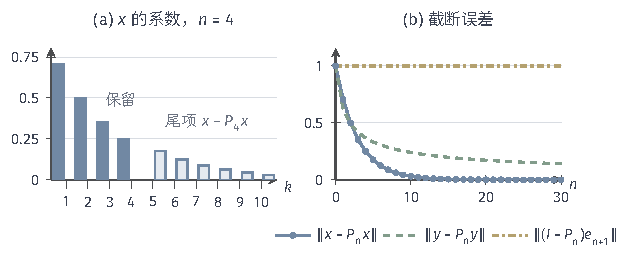
\includegraphics[width=107.2mm]{figures/02-abstract-mathematics/03-function-spaces/tikz/c2-projection-strong-norm/figure.pdf}
  \caption{截断投影的强收敛与算子范数不收敛。(a)~单位向量$x$的系数$c_k=2^{-k/2}$，$P_4$保留深色的前四项，浅色尾项构成误差$x-P_4x$；(b)~截断误差随保留项数$n$的变化：$\|x-P_nx\|=2^{-n/2}$（蓝），系数与$1/k$成比例的单位向量$y$的误差衰减较慢（绿虚线），而对被截掉的基向量$e_{n+1}$，误差始终为$1=\|I-P_n\|$（黄点划线）。}
  \label{fig:lfo-projection-strong-norm}
\end{figure}

\paragraph{有限个输入上的统一控制}
强算子收敛虽然不能控制整个单位球，对有限个输入却可以同时控制：若$x^{(1)},\ldots,x^{(m)}$是固定的输入，对每个$i$取$N_i$使误差小于$\varepsilon$，再取$N=\max_iN_i$即可。在$P_n$的例子中，失去统一控制的原因是单位球中有无穷多个相互正交的方向，每个$P_n$只能照顾其中有限个。第~\ref{sec:lfo-uniform-boundedness}节将证明，在Banach空间上，强算子收敛的算子列至少有统一的范数上界，这是算子列能被逐点控制时还剩下的统一信息。
